\section{Transparent Acceleration}
\label{sec_transacc}


Transparent acceleration of workloads is one of the design goals of
{\em Transformer}. Transparent acceleration refers to the speedup of
an application using hardware accelerators without the need of source
code access, recompilation or user intervention at run-time. We argue that such a feature is one of
the most important factors that enable the practical deployment of the
proposed heterogeneous architecture, because (1) the users'
workloads are typically present in the form of binary executables. Any
requirements on the access to source code and the capability of
rewriting the application impose tremendous obstacles for taking
advantage of a hardware accelerator; (2) the development environment
of user applications cannot be easily duplicated or emulated within
the run-time environment due to the complexity and variety of
compilers and libraries. As a result, the recompilation of an
application for hardware acceleration is either infeasible or
problematic; and (3) recompilation of user applications introduces
delays which are often unnecessary and/or intolerable. Therefore
transparent acceleration is critical for benefiting unpredictable
workloads with hardware accelerators.

To achieve transparent acceleration and ease the work of programmers,
we focus on the acceleration of commonly used libraries such as
libopenssl. Such libraries are made available with well known APIs to
their core functions, which are often the targets of acceleration. For
example, 3DES, a classic block cipher, is one of the many functions
within libopenssl, a suite of cryptography library implementing Secure
Sockets Layer (SSL) and Transport Layer Security
(TLS)\cite{wikissl} protocols. In the form of a dynamically linked
library, libopenssl provides entry points to its functions like
3DES. We propose to add a layer of wrapper functions that profiles and
intercepts the calls from user applications to the libraries that can
be accelerated with programmable logic. 


\begin{figure}
    \centering
    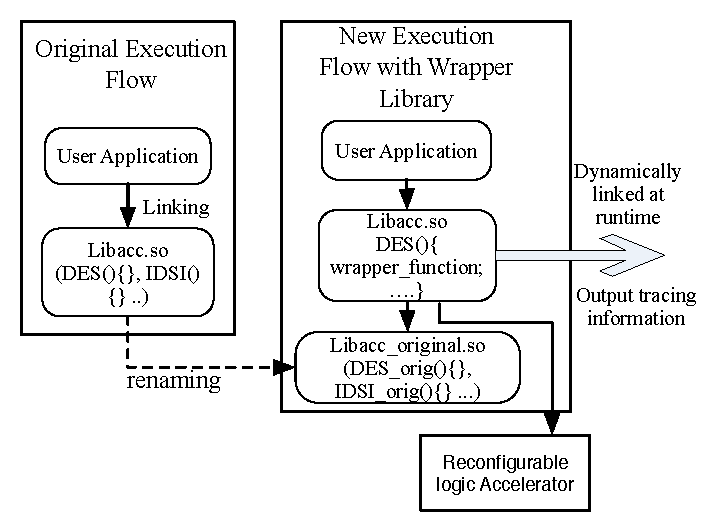
\includegraphics[width=4.0 in]{HPCA14-wrapperlib}
    \caption{Original and Modified Execution Flow}
    \label{fig_transacc_flow}
\end{figure}

Wrapper functions are presented in the form of dynamically linked
libraries, replacing the original libraries by renaming. As a result,
the calls to the original dynamic library are directed to wrapper
functions due to the linker stub \cite{linkerstub}. The modified
execution flow is shown in Figure \ref{fig_transacc_flow}.  The
original dynamic linked library is renamed by adding suffix
{\em ``\_original''}, so are its functions by rewriting its symbol table. We
create our new dynamic-linked library with the same name as the original library, and
incorporate a wrapper function to intercept all the library calls
(call to the original function names) and
redirect them to either the original software library or the hardware accelerator.

The responsibilities of wrapper functions are two folds: (1) {\em profiling}:
a wrapper library record the number of calls to each of the
library functions. Such counters reflect the demands to individual
functions (e.g. 3DES), which are used by the reconfiguration
controller to determine which functions are to be accelerated in
programmable hardware. We provide details of the algorithms for such
run-time reconfiguration in Section \ref{sec_runtime_reconfig}; and (2)
{\em function call redirection}: a wrapper function directs the
execution flow to an appropriate path, i.e. either continuing software instruction execution on a core or
acceleration with a programmable hardware unit. The wrapper functions
are aware of the currently accelerated functions on the programmable
accelerators, and such knowledge is updated by the reconfiguration
controller. If the required function is currently supported in the hardware
accelerator, this call and subsequent ones to the particular library
function(s) are redirected to the accelerator, thus reducing execution
time.

The library based transparent acceleration benefits the dynamically
linked applications which are well supported in modern operating
systems such as Windows and Linux. For statically linked applications,
although the dynamic library based transparent acceleration is limited
in detecting library calls and redirecting instruction flow to
hardware accelerators, we argue that such limitation is not inherent
to the proposed heterogeneous architecture. A user can still
incorporate our wrapper functions into the application so that the
calls to compute-intensive functions are instrumented, and the
subsequent calls are redirected to programmable accelerators when the
run-time system determines that the particular function should be sped
up with a hardware based accelerator at the current moment.
We show a sample acceleration function call process in Algorithm \ref{alg_sample_func}.

\begin{algorithm}[htb]
\scriptsize
\caption{Sample Acceleration Function Call}
\label{alg_sample_func}
\begin{algorithmic}[1]
\STATE {\em In User Function:}
\STATE {Call: DES (arg1, arg2, arg3) \newline}
\STATE {\em In Wrapper Function DES(arg1, arg2, arg3):}

\IF {DES is called}
	\STATE {RequestCounter ++ \COMMENT{Increase Request Counter by 1}}
	\IF {Request tracking time window is finished}
		\STATE{$D_{x} = \sum_{i=1}^{H}C(x,i)$ \COMMENT{Total demand}}
		\STATE{$DC_{x} = \sum_{i=1}^{H-1}(|C(x, i+1)-C(x, i)|)$\COMMENT{Demand changes}}
		\IF {Use naive scheduling}
			\STATE{$P_x = a \times D_x + (1-a) \times DC_x$ \COMMENT{Priority of this function}}
		\ENDIF
		\IF {Use Bandwidth/Speedup First scheduling}
			\STATE{$P_x = $ the result of 2D-knapsack combination}
		\ENDIF
	\ENDIF
	\IF {Function DES meets the requirement of being scheduled}
		\STATE{$ConfigStart \leftarrow 1$; $AccType \leftarrow 0$ \COMMENT{3DES is type 0}}
		\STATE {$ArgNum \leftarrow 3$; $AccPtr \leftarrow \& arg1$; $DS \leftarrow 1$}
		\IF {$ConfigDone = 1\quad\AND\quad DD = 1$}
			\STATE{$AccStart \leftarrow 1$}
		\ENDIF
		\IF {$AccDone = 1$}
			\STATE{Get back to previous thread.}
		\ENDIF
	\ELSE
		\RETURN $DES(arg1, arg2, arg3) \COMMENT{\text{Software  Version}}$
	\ENDIF
\ENDIF

\end{algorithmic}

\end{algorithm}








